\documentclass[11pt,a4paper]{article}

\usepackage[margin=1in]{geometry}
\usepackage{amsmath,amssymb,bm}
\usepackage{booktabs}
\usepackage{tikz}
\usepackage{xcolor}
\usepackage{listings}
\usepackage[hidelinks]{hyperref}
\usetikzlibrary{arrows.meta,positioning,decorations.pathreplacing}

\lstset{basicstyle=\ttfamily\small,frame=single,breaklines=true,
        columns=fullflexible,backgroundcolor=\color{black!3}}

\newcommand{\uvec}{\bm{u}}
\newcommand{\qe}{\bm{q}_{\mathrm{e}}}
\newcommand{\fexp}{f_{\mathrm{exp}}}
\newcommand{\fimp}{f_{\mathrm{imp}}}

\title{\textbf{HEVI in Jexpresso}\\[2mm]
\large Horizontally Explicit / Vertically Implicit time integration\\
for the compressible Euler equations}
\author{Jexpresso --- \texttt{src/kernel/solvers/hevi/}}
\date{}

\begin{document}
\maketitle

\noindent
Source files, in include order: \texttt{columns.jl}, \texttt{operator.jl},
\texttt{factorize.jl}, \texttt{ark.jl}, \texttt{hevi.jl},
\texttt{cfl\_diagnostics.jl}.
Worked example throughout: \texttt{problems/CompEuler/rtb\_hevi} on
\texttt{hevi\_10x1x50.msh}.

\tableofcontents

%======================================================================
\section{The problem HEVI solves}

An explicit scheme integrating the compressible Euler equations is limited by
the fastest wave on the grid: sound, at $c \approx 347$\,m/s. The constraint is
set by the \emph{sum} of the per-direction rates, because the eigenvalues of a
tensor-product operator add along its diagonal:
\begin{equation}
r_{\mathrm{exp}}
 = \frac{c}{h_\xi}+\frac{c}{h_\eta}+\frac{c}{h_\zeta}
 + \frac{\nu}{h_\xi^2}+\frac{\nu}{h_\eta^2}+\frac{\nu}{h_\zeta^2},
\qquad
\Delta t_{\max}=\frac{R}{r_{\mathrm{exp}}},
\end{equation}
with $R$ the scheme's imaginary stability radius ($3.95$ for
\texttt{CarpenterKennedy2N54}).

On an atmospheric mesh $h_\zeta \ll h_\xi$, so $c/h_\zeta$ dominates and the
whole 3D problem is stepped at a rate set by one direction. On
\texttt{hevi\_10x1x50.msh}:

\begin{center}
\begin{tabular}{lrr}
\toprule
direction & LGL spacing & acoustic limit \\
\midrule
$\xi$ ($x$)  & $172.7$\,m & $0.4976$\,s \\
$\eta$ ($y$) & $863.4$\,m & $2.488$\,s  \\
$\bm{\zeta}$ ($z$) & $\bm{34.53}$\,m & $\bm{0.09953}$\,s \\
\bottomrule
\end{tabular}
\end{center}

\noindent
HEVI removes \emph{that one term} from the explicit budget, and nothing else.

\paragraph{Consequence.} The gain is bounded by the grid's acoustic
anisotropy. On an isotropic mesh HEVI buys nothing and is strictly worse,
because the implicit tableau has a smaller explicit stability radius than a
well-tuned explicit RK. Run with \texttt{:lcfl\_report => true} first: if the
report names SGS diffusion rather than vertical acoustics as the binding term,
HEVI as built here will not help.

%======================================================================
\section{The splitting}

\subsection{Governing equations}
In conservative variables $\uvec=(\rho,\rho u,\rho v,\rho w,\rho\theta)$,
\begin{align}
\partial_t \rho + \nabla\!\cdot(\rho\bm{v}) &= 0,\\
\partial_t (\rho\bm{v}) + \nabla\!\cdot(\rho\bm{v}\otimes\bm{v}) + \nabla p
   &= -\rho g\,\hat{\bm{z}},\\
\partial_t (\rho\theta) + \nabla\!\cdot(\rho\theta\bm{v}) &= 0,
\qquad p = C_0 (\rho\theta)^{\gamma}.
\end{align}

\subsection{What is treated implicitly}
Only the terms carrying the \emph{vertical} sound wave, linearised about the
reference state $\qe$. With $\delta(\cdot)=(\cdot)-\qe$:
\begin{align}
\partial_t (\delta\rho)        &= -\partial_z\,\delta(\rho w),\\
\partial_t (\delta\rho w)      &= -\partial_z\!\big[\beta\,\delta(\rho\theta)\big] - g\,\delta\rho,\\
\partial_t (\delta\rho\theta)  &= -\partial_z\!\big[\bar\theta\,\delta(\rho w)\big],
\end{align}
with $\beta=\partial p/\partial(\rho\theta)=\gamma p/(\rho\theta)=c^2/\theta$
on the reference state. Calling this linear operator $A$,
\begin{equation}
\fimp(\uvec) = A\,(\uvec-\qe).
\end{equation}
Three of five equations are involved: the implicit variable set is
$[1,4,5]=(\rho,\rho w,\rho\theta)$, $n_{\mathrm{imp}}=3$. Horizontal momentum
stays fully explicit.

Vertical \emph{advection} deliberately stays explicit: $|w|/h_\zeta$ is
$\sim 1/800$ of $c/h_\zeta$, so making it implicit would buy nothing and would
force a refactorisation every step.

\subsection{Two properties that come free}

\paragraph{Affine-free.} $A$ acts on the deviation $\uvec-\qe$, so
$\fimp(\qe)=0$ \emph{exactly}. The reference state is an exact steady state of
the implicit part; whatever discrete hydrostatic imbalance the code already has
stays entirely inside the explicit part. The split can neither create nor
destroy balance.

\paragraph{No lost or double-counted physics.} The explicit part is not a
second, separately written RHS. It is a subtraction:
\begin{equation}
\fexp(\uvec) = \texttt{rhs!}(\uvec) - \fimp(\uvec).
\end{equation}
That costs one extra (cheap) application of $A$ per stage and guarantees that
every source term, boundary condition, SGS closure, wall model and sponge stays
exactly what the explicit code computes.

%======================================================================
\section{The IMEX Additive Runge--Kutta scheme}

\subsection{Stage equations}
An ARK method carries \emph{two} Butcher tableaux, $(a^E,b^E,c^E)$ acting on
$\fexp$ and $(a^I,b^I,c^I)$ on $\fimp$, sharing stage values:
\begin{align}
U_i &= \uvec^n + \Delta t\!\!\sum_{j<i}\! a^E_{ij}\,\fexp(U_j)
                + \Delta t\!\!\sum_{j\le i}\! a^I_{ij}\,\fimp(U_j),\\
\uvec^{n+1} &= \uvec^n + \Delta t\sum_i b^E_i\,\fexp(U_i)
                       + \Delta t\sum_i b^I_i\,\fimp(U_i).
\end{align}
$a^I$ is lower triangular \emph{including} the diagonal ($a^I_{ii}=\gamma$), so
each stage needs one linear solve
\begin{equation}
\big(I-\gamma\Delta t\,A\big)\,(U_i-\qe) = \mathrm{tmp}_i-\qe ,
\label{eq:solve}
\end{equation}
while $a^E$ is strictly lower triangular, so $\fexp$ is never solved for.

\subsection{The default tableau: ARS232}
With $\gamma=(2-\sqrt2)/2$ and $\delta=-2\sqrt2/3$,
\begin{equation}
a^E=\begin{pmatrix}0&0&0\\ \gamma&0&0\\ \delta&1-\delta&0\end{pmatrix},
\qquad
a^I=\begin{pmatrix}0&0&0\\ 0&\gamma&0\\ 0&1-\gamma&\gamma\end{pmatrix},
\qquad
b^E=b^I=\begin{pmatrix}0\\ 1-\gamma\\ \gamma\end{pmatrix}.
\end{equation}
Three stages, second order, \textbf{stiffly accurate}
($b^I=a^I_{s,:}$, $b^E=a^E_{s,:}$), so the last stage \emph{is} the answer and
its RHS evaluation is reused as the next step's FSAL. Net cost:
\textbf{3 \texttt{rhs!} evaluations and 2 column solves per step}, against
\texttt{CarpenterKennedy2N54}'s 5 \texttt{rhs!}.

Available: \texttt{:ARS111 :ARS121 :ARS122 :ARS222 :ARS232 :ARS343 :ARS443}.

%======================================================================
\section{Joint stability --- the part that matters}

\subsection{Why the usual figure of merit is wrong}
A tableau is normally chosen by its \emph{explicit imaginary radius}. For HEVI
that is the wrong number, and choosing on it is an active trap.

A HEVI acoustic mode with horizontal wavenumber $k_x$ and vertical $k_z$ loads
\emph{both} halves at once:
\begin{equation}
z_E = \mathrm{i}\,\Delta t\,c\,k_x, \qquad
z_I = \mathrm{i}\,\Delta t\,c\,k_z .
\end{equation}
Stability requires the \emph{joint} amplification factor to stay bounded over
the whole rectangle, not merely along the edge $z_I=0$:
\begin{equation}
\boxed{\;
R(z_E,z_I)=1+\big(z_E\,b^{E\top}+z_I\,b^{I\top}\big)
\big(I-z_E a^E-z_I a^I\big)^{-1}\bm{1}\;}
\label{eq:joint}
\end{equation}
\texttt{ark\_joint\_amplification} samples $\max|R|$ over that rectangle;
\texttt{ark\_joint\_dt\_max} inverts it for $\Delta t$.

\subsection{The ARS343 trap, measured}
On the anisotropic \texttt{rtb} mesh:
\begin{center}
\begin{tabular}{lccc}
\toprule
tableau & RHS/step & explicit imag.\ radius & joint $\Delta t_{\max}$ \\
\midrule
ARS232 & 3 & $1.732$ & $\bm{0.052}$\,s \\
ARS443 & 4 & $1.570$ & $0.059$\,s \\
ARS343 & 4 & $\bm{2.828}$ (best) & $\bm{0.0004}$\,s \\
\bottomrule
\end{tabular}
\end{center}
ARS343 has the \emph{largest} explicit imaginary radius in the family and a
joint region $\sim\!130\times$ smaller. This case shipped on ARS343 at
$\Delta t=0.03$ and amplified $0.79\,\%$/s --- slow enough to look like
anything but a tableau problem: it presented as a blow-up at a fixed
\emph{model} time, nearly independent of $\Delta t$, that moved with the rank
count.

\begin{quote}
\textbf{Judge a tableau by \eqref{eq:joint}, never by the explicit radius.}
A check sampling only $z_I=0$ passes ARS343.
\texttt{test/hevi/test\_joint\_stability.jl} pins exactly that trap.
\end{quote}

\subsection{The startup guard}
\texttt{build\_hevi} evaluates $\max|R|$ at the deck's actual $\Delta t$ on the
actual mesh and \textbf{refuses to start} if it exceeds $1$, naming the neutral
limit, a recommended step ($70\,\%$ of it) and the tableaux whose joint region
does cover the mesh. Override with \texttt{:hevi\_verify => false}. On
\texttt{hevi\_10x1x50.msh}:
\begin{lstlisting}
joint IMEX stability: explicit half 3.7 1/s, implicit half 14.4 1/s
    dt_max here = 0.3567 s     (recommended: 0.2497 s, i.e. 70%)
\end{lstlisting}
against an explicit acoustic limit of $0.0995$\,s --- consistent with explicit
diverging at $\Delta t=0.25$ while HEVI runs.

%======================================================================
\section{The column solve}

\subsection{Why it is cheap}
$A$ couples a node only to nodes in the \emph{same vertical column}, and only
within $\pm(n_{\mathrm{gl}}-1)$ levels: inside an element the $\zeta$
collocation derivative reaches all $n_{\mathrm{gl}}$ nodes of the line, and DSS
links an element only to those directly above and below. So
$(I-\gamma\Delta t A)$ is block-banded per column and a direct banded LU costs
nothing next to one explicit RHS.

For \texttt{rtb\_hevi} ($\mathrm{nop}=4\Rightarrow n_{\mathrm{gl}}=5$, 50
vertical elements):
\begin{center}
\begin{tabular}{ll}
\toprule
columns & $205$ globally $=(10\cdot4+1)\times(1\cdot4+1)=41\times5$\\
levels per column & $201 = 50\cdot4+1$\\
matrix order $n$ & $603 = 201\times n_{\mathrm{imp}}$\\
bandwidth $k_l=k_u$ & $14 = n_{\mathrm{imp}}(n_{\mathrm{gl}}-1)+2$\\
storage & $41.5$\,MB on the busiest rank\\
\bottomrule
\end{tabular}
\end{center}

\subsection{The matrix is extracted, not derived}
The band is recovered by \emph{probing}. Colour the levels modulo
$S=2(n_{\mathrm{gl}}-1)+1=9$. A probe that is $1$ on one colour and $0$
elsewhere hits, for each row, exactly one column of the band --- the window a
row can see is $S$ wide, so it contains exactly one level of any given colour.
Hence $S\cdot n_{\mathrm{imp}}=27$ applications of $A$ recover every entry
exactly.

Deriving them by hand would mean keeping the $\zeta$ collocation weights,
metric terms, DSS sum, inverse mass matrix and wall-flux condition in sync
manually. A discrepancy would \emph{not} break a convergence test --- the split
stays consistent whatever the implicit matrix is, since
$\fexp=\texttt{rhs!}-\fimp$ --- it would silently make the solve approximate and
bring the vertical acoustic CFL back with nothing in the output to say why.
Probing removes that failure mode: \textbf{the matrix is the operator, by
construction}.

\subsection{One factorisation per run}
$\gamma$ is fixed by the tableau and $\Delta t$ is fixed, so $\gamma\Delta t$ is
constant and \eqref{eq:solve} is factorised \emph{once} at setup.

\subsection{Under MPI}
A column-local solve assumes each column lives on one rank. p4est partitions by
Morton order, so that holds only at tree-column granularity.
\texttt{columns.jl} makes it work under any partition: rank-local columns are
solved in place with no communication; split columns are gathered onto an
owner, solved, and scattered back. The setup report prints how many columns are
split --- typically $0\,\%$ with \texttt{:lxy\_partition => true} and up to
$100\,\%$ under p4est, which is correct but communication-heavy. HEVI therefore
defaults to the columnar partition, and \texttt{:linitial\_refine => true}
forces p4est and gives that up.

%======================================================================
\section{Worked example: \texttt{rtb\_hevi}}

\begin{figure}[h]
\centering
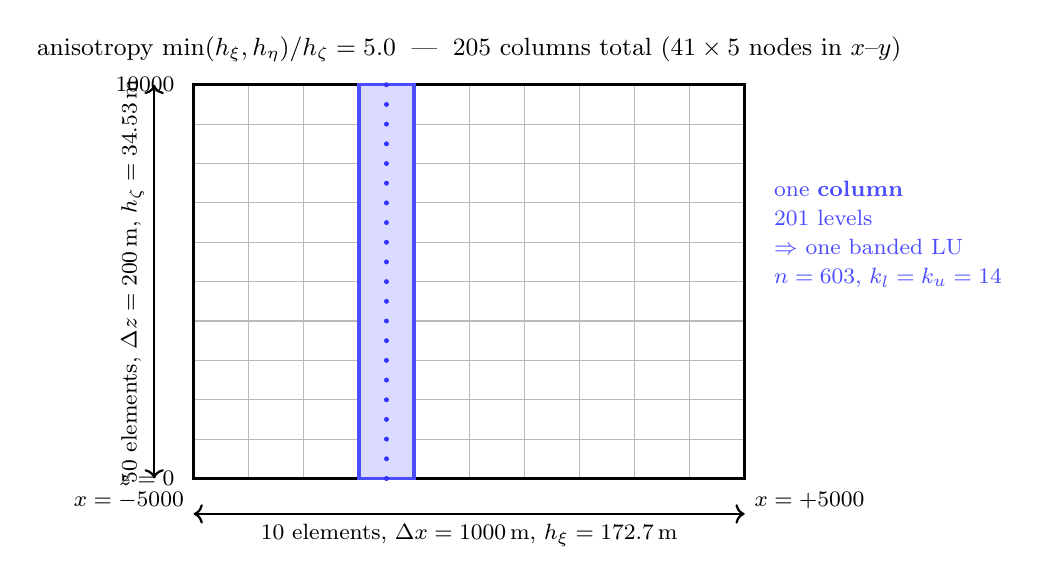
\begin{tikzpicture}[scale=1.0]
  \def\W{7.0}   % drawing width
  \def\H{5.0}   % drawing height
  \pgfmathsetmacro{\dx}{\W/10}

  % vertical element lines (10 columns of elements)
  \foreach \i in {0,...,10}{
    \draw[gray!55] (\i*\dx,0) -- (\i*\dx,\H);
  }
  % horizontal element lines: 50 elements, draw every 5th for legibility
  \foreach \j in {0,...,10}{
    \draw[gray!55] (0,\j*\H/10) -- (\W,\j*\H/10);
  }
  \draw[very thick] (0,0) rectangle (\W,\H);

  % highlight one column
  \fill[blue!14] (3*\dx,0) rectangle (4*\dx,\H);
  \draw[blue!70,very thick] (3*\dx,0) rectangle (4*\dx,\H);
  \foreach \j in {0,...,20}{
    \fill[blue!80] (3.5*\dx,\j*\H/20) circle (0.9pt);
  }

  % annotations
  \node[blue!70,right,align=left] at (\W+0.25,\H*0.62)
    {\footnotesize one \textbf{column}\\[-0.5mm]
     \footnotesize 201 levels\\[-0.5mm]
     \footnotesize $\Rightarrow$ one banded LU\\[-0.5mm]
     \footnotesize $n=603$, $k_l=k_u=14$};

  \draw[<->,thick] (0,-0.45) -- (\W,-0.45)
     node[midway,below]{\footnotesize 10 elements, $\Delta x=1000$\,m, $h_\xi=172.7$\,m};
  \draw[<->,thick] (-0.5,0) -- (-0.5,\H)
     node[midway,left,rotate=90,anchor=south]{\footnotesize 50 elements, $\Delta z=200$\,m, $h_\zeta=34.53$\,m};

  \node[below left] at (0,-0.05) {\footnotesize $x=-5000$};
  \node[below right] at (\W,-0.05) {\footnotesize $x=+5000$};
  \node[left] at (-0.12,0) {\footnotesize $z=0$};
  \node[left] at (-0.12,\H) {\footnotesize $10000$};

  \node[align=center] at (\W/2,\H+0.45)
    {\small anisotropy $\min(h_\xi,h_\eta)/h_\zeta = 5.0$
     \;---\; 205 columns total ($41\times5$ nodes in $x$--$y$)};
\end{tikzpicture}
\caption{\texttt{hevi\_10x1x50.msh}. Horizontal element lines are drawn every
fifth element for legibility. Each vertical line of nodes (one highlighted) is
an \emph{independent} banded system; horizontally nothing is coupled
implicitly.}
\end{figure}

\subsection{Measured, 1 rank}
\begin{center}
\begin{tabular}{lcc}
\toprule
 & explicit (CK2N54) & HEVI (ARS232)\\
\midrule
stability limit on $\Delta t$ & $0.0995$\,s (acoustic $\zeta$) & $\bm{0.3567}$\,s (joint)\\
observed & diverges at $\Delta t=0.25$ & runs at $\Delta t=0.25$\\
cost per step & $0.212$\,s & $\bm{0.156}$\,s\\
RHS evaluations per step & 5 & 3 ($+$2 column solves)\\
\bottomrule
\end{tabular}
\end{center}
HEVI is cheaper \emph{per step} here \emph{and} admits a larger step. Comparing
the two at the \emph{same} $\Delta t$ measures only per-step cost and says
nothing about the method --- the gain lives in the step size.

\subsection{Setup self-check}
\begin{lstlisting}
self-check: band matches operator to 4.07e-16; solve residual 2.78e-15
\end{lstlisting}

%======================================================================
\section{Reading the CFL report}
\begin{lstlisting}
 |  dt gain available, per scheme (rate-summed, before per-stage cost):
 |    HEVI  (vertical acoustics implicit)              4.82x
 |    HEVI + implicit vertical diffusion               5.24x
 |    HEVI + acoustic substepping (outer step)        58.06x
\end{lstlisting}
These are \textbf{$\Delta t$-ratio upper bounds}, obtained by summing
per-direction stability rates and removing the terms each scheme would make
implicit, $\text{gain}=r_{\mathrm{full}}/r_{\mathrm{scheme}}$. They are
\emph{not} wall-clock speedups, and they are idealisations: the realised limit
comes from the joint IMEX region, which also pays for ARS232's smaller explicit
radius. On this mesh the first line reads $4.82\times$ while the joint
calculation gives $0.3567/0.0995=3.6\times$.

\begin{quote}
\textbf{Only the first line corresponds to an implemented scheme.} Vertical
diffusion is not in the implicit operator, and acoustic substepping is not
implemented.
\end{quote}

%======================================================================
\section{Deck options}
\begin{lstlisting}
:ode_solver     => HEVI_ARK(:ARS232),   # instead of CarpenterKennedy2N54()
:dt             => 0.19,

:hevi_verify    => true,      # setup self-check + stability guard (default)
:hevi_wall_flux => true,      # zero implicit vertical mass flux at floor/lid
:hevi_vars      => [1,4,5],   # override the implicit variable set
:lcfl_report    => true,      # print the stability table at startup
:lxy_partition  => true,      # columnar partition (HEVI default)
\end{lstlisting}
\texttt{:ladapt => true} is refused: adaptation invalidates the column
topology, the factorised column matrices and the gather/scatter plan.

%======================================================================
\section{Limitations}
\begin{itemize}
\item \textbf{Bounded by acoustic anisotropy.} Removes the vertical acoustic
      term and nothing else; on an isotropic mesh HEVI is slower than explicit.
\item \textbf{Horizontal acoustics stay explicit.} Getting past the anisotropy
      ratio needs acoustic substepping or a full 3D implicit solve.
      \emph{(Not implemented.)}
\item \textbf{Vertical diffusion stays explicit.} If the CFL report names SGS
      diffusion as the binding term, this split will not help.
      \emph{(Not implemented.)}
\item \textbf{Fixed step.} The tableaux carry no embedded error estimator.
\item \textbf{No AMR.}
\end{itemize}

\end{document}
